\documentclass[]{../template/Report}%方括号内写yuxi即生成预习报告\documentclass[yuxi]{../template/Report}
\settemplatedir{../template/}%设置模板路径
\sisetup{
    separate-uncertainty = true,
    per-mode = symbol
}

\exname{棱镜偏向角特性} %实验名称
\extable{} %实验桌号
\instructor{} %指导教师
\class{} %班级
\name{} %姓名
\stuid{} %学号

\nyear{} %年
\nmonth{} %月
\nday{} %日
\nweekday{} %星期几，e.g. \nweekday{三}
\daypart{}%上午/下午

\redate{} %如有实验补做，补做日期
\resitu{} %情况说明：

\begin{document}
\maketitle%输出封面

\section{预习报告（10分）}
（注：将已经写好的“物理实验预习报告”内容拷贝过来）

\subsection{实验综述（5分）}
（自述实验现象、实验原理和实验方法，包括必要的光路图、电路图、公式等。不超过500字。）
\subsubsection{实验步骤}
1）调整分光计
\par
2）测量三棱镜顶角$\angle A$
\par
3）测量最小偏向角$\delta_{\text min}$
\par
4）计算三棱镜单色光折射率
\par
5）绘制色散曲线并思考
\par
\begin{figure}[H]
    \centering
    
\includegraphics[width=0.6\textwidth]{实验步骤.png}
    \caption{实验步骤}
\end{figure}

\subsubsection{实验原理}
\textbf{(1)偏向角与最小偏向角的形成：}
\par
当一束平行单色光入射到三棱镜的光学面时，光线会经两次折射后从另一光学面出射，出射光线相对于入射光线的偏折角度称为偏向角$\delta$。实验中通过转动三棱镜改变入射角，可观察到偏向角随入射角的变化而变化，当入射角等于出射角时，偏向角达到最小值，称为最小偏向角$\delta_{\text min}$。此时，棱镜内的折射光线与棱镜底边平行，是计算棱镜折射率的关键条件。
\par

\textbf{(2)折射率的计算原理：}
\par
利用最小偏向角可推导棱镜对单色光的折射率公式。设棱镜顶角为$\alpha$，根据折射定律及几何关系，折射率$\eta $满足：
\begin{center}
$\eta = \frac{\sin (\frac{\alpha + \delta_{\text min}}{2})}{\sin (\frac{\alpha}{2})}$
\end{center}
\par
通过分光计测量棱镜顶角$\alpha$和某波长光的最小偏向角$\delta_{\text min}$，代入上式即可求出该波长对应的折射率$\eta $。

\begin{figure}[H]
    \centering
    
\includegraphics[width=0.6\textwidth]{实验原理.png}
    \caption{实验原理}
\end{figure}


\subsection{实验重点（3分）}
（简述本实验的学习重点，不超过100字。）
\par
(1)\textbf{分光计调整和使用}
\par
(2)\textbf{三棱镜顶角的测量}
\par
(3)\textbf{测量棱镜的折射率并研究其色散规律}


\subsection{实验难点（2分）}
（简述本实验的实现难点，不超过100字。）
\par
(1)\textbf{分光计的精确调整：}实验需完成目镜调焦（使叉丝清晰）、物镜调焦（使反射像清晰无视差）、载物台与望远镜同轴等高等多步骤调节，任何一步偏差都会导致后续测量误差。
\par
(2)\textbf{最小偏向角的准确识别与测量：}需通过转动载物台找到偏向角最小位置，此时谱线随载物台转动的移动方向会发生逆转，判断转折点易受主观误差影响。
\par
(3)\textbf{三棱镜顶角测量的对准误差：}采用反射法或折射法测量顶角时，需使棱镜顶角对准平行光管，且望远镜需分别捕捉两侧反射光，角度对准偏差会直接影响顶角测量精度。
\par
(4)\textbf{注意事项：}光学元件，轻拿轻放，勿用手触摸光学面；刻度盘读数过0°/360°时，注意修正；汞灯辐射紫外线较强，不要眼睛直视汞灯；分光计调整时，带眼镜的同学要注意镜片不要碰到目镜；眼镜如有防蓝光功能，可能没法看到紫光。
\par


\begin{fullreportonly}
\section{原始数据（20分）}
（将有老师签名的“自备数据记录草稿纸”的扫描或手机拍摄图粘贴在下方，完整保留姓名，学号，教师签字和日期。）
% \begin{figure}[H]
%     \centering
%     
\includegraphics[width=0.6\textwidth]{figures/原始数据.jpg}
%     \caption{原始数据}
% \end{figure}

\section{结果与分析（60分）}
\subsection{数据处理与结果（30分）}
（列出数据表格、选择适合的数据处理方法、写出测量或计算结果。）

\subsubsection{实验一：测量三棱镜顶角}
\begin{table}[H]
    \centering
    \caption{实验一测量三棱镜顶角}
    \begin{tabular}{|c|c|c|c|c|c|}
        \hline
        \textbf{棱脊分光法} & 
        \multicolumn{2}{|c|}{\textbf{左位置}} &
        \multicolumn{2}{|c|}{\textbf{右位置}} &
        \textbf{$\angle A$}  \\
        \hline
        \textbf{测量次数} & \textbf{游标1$(\theta_1)$} & \textbf{游标2$(\theta_2)$} & \textbf{游标1$(\theta_{10})$} & \textbf{游标2$(\theta_{20})$} & \textbf{$\frac{1}{4}(|\theta_1 - \theta_{10}| + |\theta_2 - \theta_{20}|)$}  \\
        \hline
        1 & \ang{330;52} & \ang{150;48} & \ang{210;54} & \ang{30;55} & \ang{59;58}  \\
        \hline
        2 & \ang{354;0} & \ang{173;57} & \ang{234;0} & \ang{54;6} & \ang{59;58}  \\
        \hline
        3 & \ang{282;32} & \ang{102;33} & \ang{162;27} & \ang{342;30} & \ang{60;1}  \\
        \hline
        4 & \ang{310;45} & \ang{130;42} & \ang{190;53} & \ang{10;54} & \ang{59;55}  \\
        \hline
        5 & \ang{343;30} & \ang{163;26} & \ang{223;31} & \ang{43;33} & \ang{59;58}  \\
        \hline
        6 & \ang{6;44} & \ang{186;46} & \ang{246;51} & \ang{66;51} & \ang{60;0}  \\
        \hline
    \end{tabular}
\end{table}
$\angle A$平均值：$\bar{\angle A} = \frac{\displaystyle\sum_{i=1}^6 \angle A_i}{6} = \ang{59;58}$

\subsubsection{实验二：测量三棱镜对汞灯绿光的最小偏向角}
\begin{table}[H]
    \centering
    \caption{实验二测量三棱镜对汞灯绿光的最小偏向角}
    \begin{tabular}{|c|c|c|c|c|c|}
        \hline
         & 
        \multicolumn{2}{|c|}{\textbf{$\varphi_{min}$}} &
        \multicolumn{2}{|c|}{\textbf{$\varphi_{0}$}} &
        \textbf{最小偏向角$\delta_{min}$}  \\
        \hline
        \textbf{测量次数} & \textbf{游标1$(\varphi _1)$} & \textbf{游标2$(\varphi _2)$} & \textbf{游标1$(\varphi_{10})$} & \textbf{游标2$(\varphi_{20})$} & \textbf{$\frac{1}{2}(|\varphi_1 - \varphi_{10}| + |\varphi_2 - \varphi_{20}|)$}  \\
        \hline
        1 & \ang{247;45} & \ang{67;45} & \ang{302;30} & \ang{122;26} & \ang{54;43}  \\
        \hline
        2 & \ang{220;28} & \ang{40;30} & \ang{277;2} & \ang{97;3} & \ang{56;34}  \\
        \hline
        3 & \ang{237;22} & \ang{57;22} & \ang{294;8} & \ang{114;4} & \ang{56;44}  \\
        \hline
        4 & \ang{254;12} & \ang{74;10} & \ang{311;45} & \ang{131;40} & \ang{57;32}  \\
        \hline
        5 & \ang{226;48} & \ang{46;50} & \ang{281;23} & \ang{101;23} & \ang{54;34}  \\
        \hline
        6 & \ang{159;50} & \ang{339;54} & \ang{214;2} & \ang{34;10} & \ang{54;14}  \\
        \hline
    \end{tabular}
\end{table}
$\delta_{min}$平均值：$\bar{\delta_{min}} = \frac{\displaystyle\sum_{i=1}^6 \delta_{min}i}{6} = \ang{55;44}$


\subsubsection{实验三：计算汞灯单色光折射率}
\begin{table}
    \centering
    \caption{实验三数据记录}
    \begin{tabular}{|c|c|c|c|c|c|}
        \hline
         & 
        \multicolumn{2}{|c|}{\textbf{$\varphi_{min}$}} &
        \multicolumn{2}{|c|}{\textbf{$\varphi_{0}$}} &
        \textbf{最小偏向角$\delta_{min}$}  \\
        \hline
        \textbf{汞灯单色光} & \textbf{游标1$(\varphi _1)$} & \textbf{游标2$(\varphi _2)$} & \textbf{游标1$(\varphi_{10})$} & \textbf{游标2$(\varphi_{20})$} & \textbf{$\frac{1}{2}(|\varphi_1 - \varphi_{10}| + |\varphi_2 - \varphi_{20}|)$}  \\
        \hline 
        \textbf{紫} & \ang{155;46} & \ang{335;50} & \ang{214;6} & \ang{34;10} & \ang{58;20}  \\
        \hline
        \textbf{蓝} & \ang{157;6} & \ang{337;12} & \ang{214;6} & \ang{34;10} & \ang{56;59}  \\
        \hline
        \textbf{黄} & \ang{160;16} & \ang{340;20} & \ang{214;6} & \ang{34;10} & \ang{53;50}  \\
        \hline
    \end{tabular}
\end{table}
折射率计算公式：
\[
    \eta = \frac{\sin (\frac{\angle A + \delta_{min}}{2})}{\sin (\frac{\angle A}{2})}
\]
\begin{table}[H]
    \centering
    \caption{实验三计算汞灯单色光折射率}
    \begin{tabular}{|c|c|c|c|}
        \hline
        \textbf{汞灯单色光波长} & \textbf{$\angle A$} & \textbf{$\delta_{min}$} & \textbf{$\eta$}  \\
        \hline
        \textbf{404.7nm（紫）} & \ang{59;58} & \ang{58;20} &  1.7183  \\
        \hline
        \textbf{435.8nm（蓝）} & \ang{59;58} & \ang{56;59} &  1.7060  \\
        \hline
        \textbf{546.0nm（绿）} & \ang{59;58} & \ang{55;44} &  1.6946  \\
        \hline
        \textbf{577.1nm（黄）} & \ang{59;58} & \ang{53;50} &  1.6767  \\
        \hline
    \end{tabular}
\end{table}
\begin{figure}[H]
    \centering
    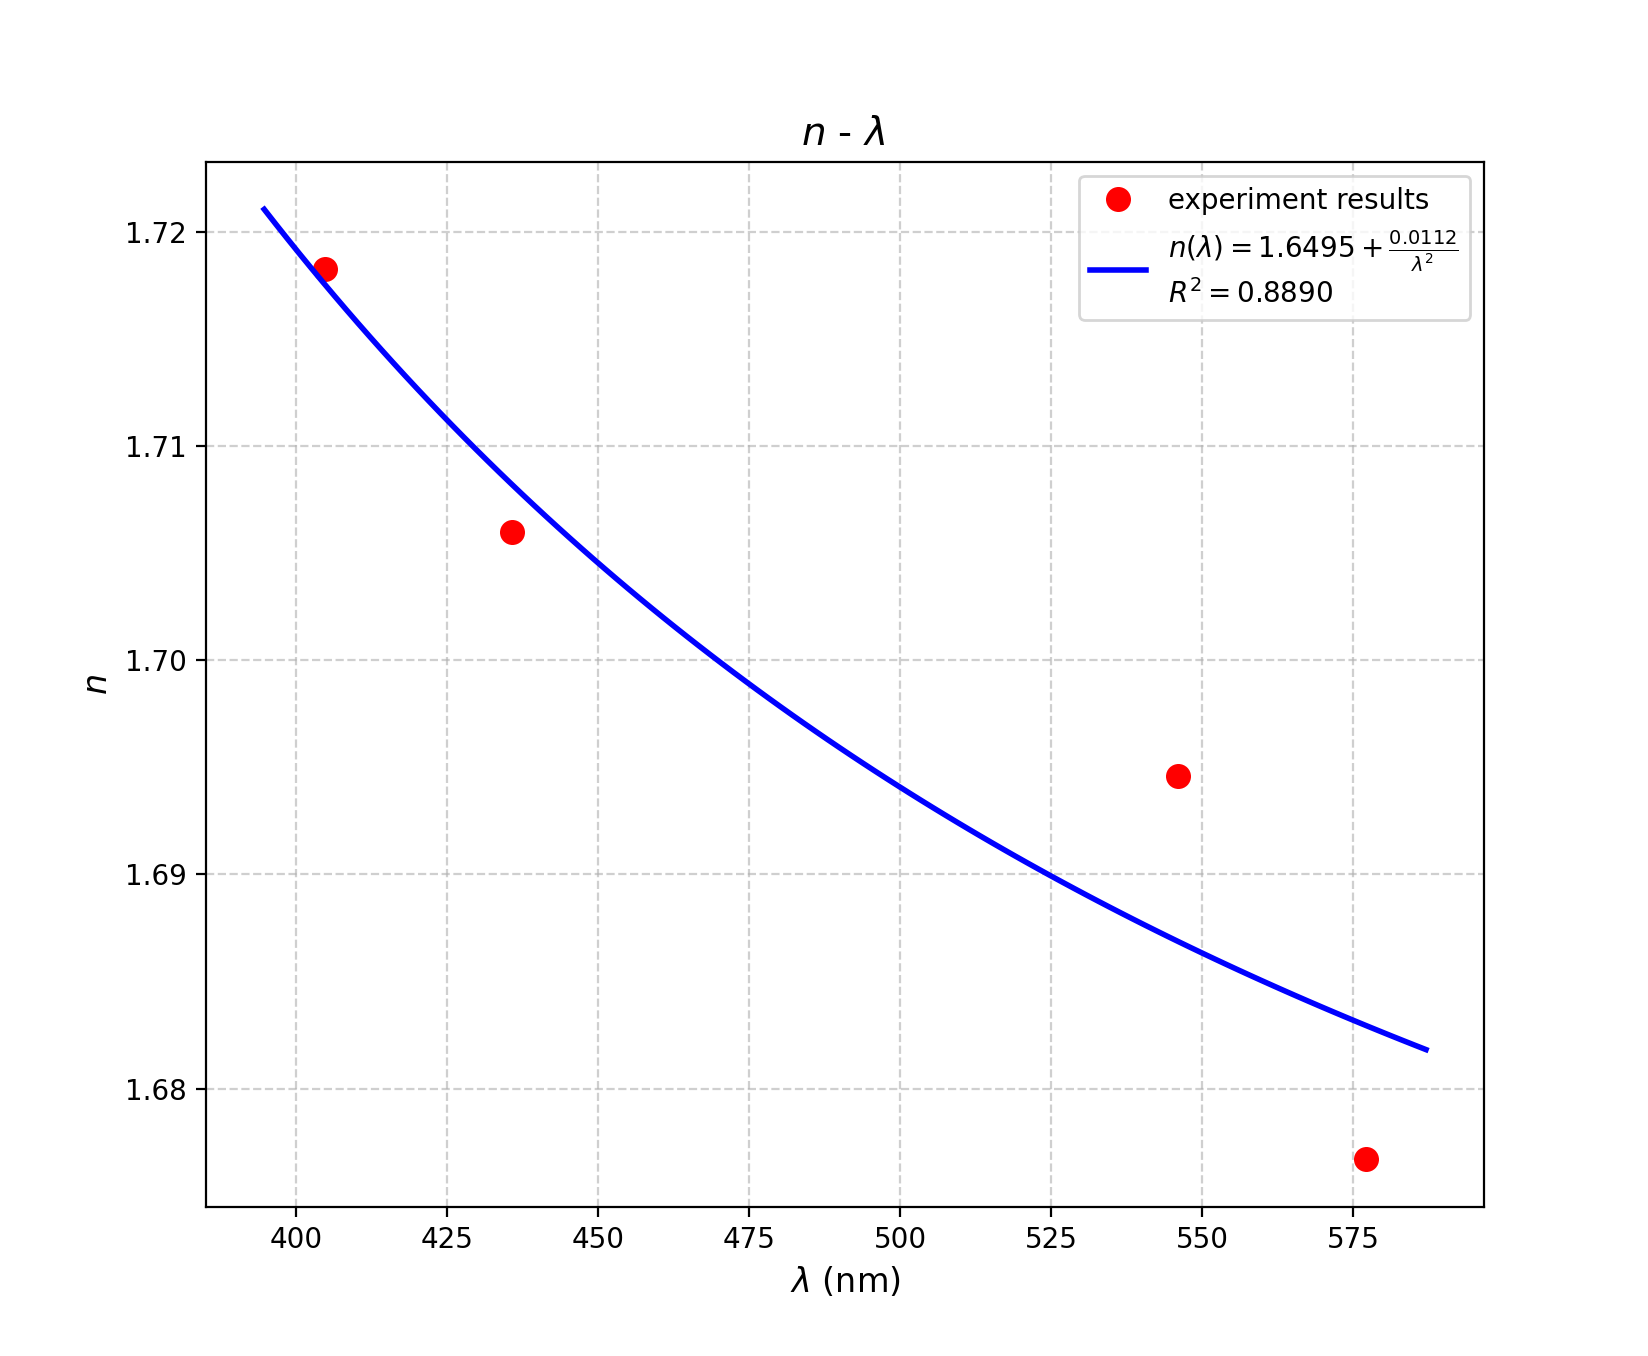
\includegraphics[width=0.6\textwidth]{figures/数据拟合.png}
    \caption{$\eta - \lambda$ 拟合图象}
\end{figure}

\subsection{误差分析（20分）}
（运用测量误差、相对误差或不确定度等分析实验结果，写出完整的结果表达式，并分析误差原因。）
\subsubsection{仪器调整相关误差：分光计调整不完善}
\textbf{(1)载物台与主轴不垂直：}棱镜光学面法线与主轴不平行，引起反射/折射光线偏移，测量角度产生系统误差。
\par
\textbf{(2)平行光管未校准：}出射光非平行光，导致偏向角测量精度下降。

\subsubsection{测量操作相关误差}
\textbf{(1)最小偏向角判断误差：}实验中需转动望远镜寻找最小偏向角位置，若未精确找到光线反向移动的临界点，会导致偏向角测量值偏大。
\par
\textbf{(2)棱镜放置误差：}棱镜光学面未与入射光保持合理角度，或棱脊未对准平行光管狭缝，导致入射光未完全照射到光学面，影响偏向角稳定性。
\par
\textbf{(3)读数误差：}游标卡尺精度限制或人为估读偏差，直接引入随机误差。

\subsubsection{外界干扰因素}
\textbf{(1)温度影响：}环境温度改变导致棱镜折射率变化，间接影响偏向角测量值。
\par
\textbf{(2)气流影响：}实验环境气流波动干扰光路，使光斑抖动，增加读数不确定性。



\subsection{实验探讨（10分）}
（对实验内容、现象和过程的小结，不超过100字。）
\par
通过本次实验，我巩固了分光计调整和使用，熟练了三棱镜顶角的测量，学会了测量棱镜的折射率并研究了其色散规律。
\par
本次实验中，旋转目镜、观察成像、左右两次读数等等步骤，都需要我们严谨、认真、耐心的态度。最后的实验数据处理，也需要我们掌握python/matlab对数据进行拟合分析。



\section{思考题（10分）}
（解答教材或讲义或老师布置的思考题，请先写题干，再作答。）
\subsection{测量时如何识别最小偏向角$\delta$的位置？}
偏向角随入射角增大先减小后增大，转折点对应最小偏向角。具体步骤如下：
\par
\textbf{(1)}将三棱镜放置在载物台上，使平行光管入射光射向棱镜光学面，望远镜从出射光方向观察，找到清晰的汞单色光谱线。
\par
\textbf{(2)}缓慢转动载物平台，同时观察望远镜中单色谱线的移动方向。当谱线移动到某一位置后突然向反方向移动，表明偏向角$\delta$开始增大。
\par
\textbf{(3)}谱线移动方向发生反向转折的临界点，即为该单色光的最小偏向角$\delta$位置。此时需固定载物台，将望远镜分划板对准该谱线，记录分光计读数。
\subsection{设计一种测量三棱镜折射率的方法}
\textbf{掠入射法}
\par
原理：利用扩展光源照射三棱镜光学面，通过观察出射光的明暗分界线确定极限出射角，结合折射定律计算折射率。
\par
实验步骤：
\par
(1)分光计调整：调节望远镜聚焦无穷远，平行光管出射平行光，载物台水平。
\par
(2)放置三棱镜：将三棱镜置于载物台，使光学面AB与平行光管光轴成一定角度，扩展光对准AB面。
\par
(3)寻找极限出射角：从AC面用望远镜观察，找到半明半暗视场的分界线，记录游标读数$\theta_1、\theta_2$。
\par
(4)测量AC面法线位置：转动望远镜至AC面法线方向，记录读数$\theta_1'$、$\theta_2'$，计算出射极限角$\psi = |(\theta_1 - \theta_1') + (\theta_2 - \theta_2')|/2$
\par
(5)计算折射率：
\[
    \eta = \sqrt{1 + (\frac{\cos \angle A + \sin \psi }{\sin \angle A})^2} 
\]
\end{fullreportonly}
\insertnotes
\end{document}